The definition of the JSR is generalized as follows for constrained systems.
\begin{definition}[\cite{dai2012gel}]
  \label{def:cjsr}
  The \emph{constrained joint spectral radius} (CJSR) of
  \defAG{}, denoted as $\cjsr$,
  is
  \begin{equation}
    \label{eq:jsrtheo}
    \limsup_{k \to \infty} \cjsrrk = \cjsr = \lim_{k \to \infty} \cjsrk
  \end{equation}
  where
  \begin{equation}
    \label{eq:cjsrrk}
    \cjsrrk
    = \max \big\{\, \jsrc : c \in \G_k, c \text{ is a cycle}\,\big\}, \quad \jsrc = [\rho(A_c)]^{1/k},
  \end{equation}
  and
  \begin{equation}
    \label{eq:cjsrk}
    \cjsrk =
    \max \big\{\, \|A_s\|^{1/k}\\: s \in \G_k \,\big\}.
  \end{equation}
\end{definition}


We can readily see that
\(
  \cjsrrk \leq \cjsrk
\)
for any $k$ and \emph{submultiplicative}\footnote{A matrix norm $\norm{\cdot}$ is \emph{submultiplicative} if $\norm{AB} \leq \norm{A} \cdot \norm{B}$ for all matrices $A$ and $B$.} norm $\norm{\cdot}$.
Equality \eqref{eq:jsrtheo} is called the \emph{Joint Spectral Radius Theorem} and was proved in 1992 by Berger and Wang~\cite{berger1992bounded} in the unconstrained case.
Elsner~\cite{elsner1995generalized} provided a somewhat simpler self contained proof in 1995.
Both proofs use rather involved results on the joint spectral radius.
In the general constrained case, the equality \eqref{eq:jsrtheo}
was first proved in \cite{dai2012gel} with the help of heavy-weighted machinery
of ergodic theory, and later simpler proofs appeared.

A popular method for proving stability of a dynamical system is to find a Lyapunov function.
In this section, we introduce measures playing a role dual to Lyapunov function for switched system.
These measures provide a certificate for instability.
Finding Lyapunov functions and finding these measures are in fact two dual programs, %
they are respectively provided by \progref{primalinf} and \progref{dualinf}.
We will be succinct in our definition of measure-theoretic concepts but the interested reader can find an good introduction to writing programs using measures and functions as decision variables in \cite{Lasserre2009}.

Consider the dual pair $(\Fb, \Fbd)$ where $\Fb$ is the space of bounded measurable
functions on $\Sn = \{\, x \in \R^n : \norm{x}_2 = 1 \,\}$ where $\norm{\cdot}_2$ is the \emph{Euclidean} norm, $\Fbd$ is the space of \emph{finite}\footnote{The measure $\mu$ is \emph{finite} if $\mu(\Sn)$ is finite.} \emph{signed}\footnote{A \emph{signed} measure is a difference between two measures, i.e. $\mu - \nu$ where $\mu$ and $\nu$ are measures is a signed measure.} Borel measures on $\Sn$ and the scalar product between a function $f \in \Fb$ and a measure $\mu \in \Fbd$ is $\langle f, \mu \rangle = \int f \dif \mu$.
Given a function $f(x) \in \Fb$, we can define the homogeneous\footnote{A function $f$ is homogeneous if $f(\alpha x) = \alpha f(x)$ for any scalar value $\alpha$.}
function $h(f) \eqdef x \mapsto \|x\|_2f(x/\|x\|_2)$ on $\R^n$.
We define $\F = \{\, h(f) \mid f \in \Fb \,\}$ with the scalar product $\la h(f), \mu \ra = \la f, \mu \ra$ for $f \in \Fb, \mu \in \Fbd$.

Given an application $A$ and a measure $\mu \in \Fbd$,
the \emph{pushforward measure} $\pushf{A}{\mu}$ is often defined to be the measure given by
$(\pushf{A}{\mu})(B) = \mu(A^{-1}(B))$ for $B \in \Sn$.
However, since $\Sn$ may not be invariant under application of the matrices of $\A$,
we will use an alternative definition.
Given an application $A$ and a measure $\mu$,
the pushforward measure $\pushf{A}{\mu}$ is defined to be the measure such that
$\la f, \pushf{A}{\mu} \ra = \la f \circ A, \mu \ra$ for any $f \in \F$.
Moreover, given $B \subseteq \Sn$, we define $\mu(B) = \la h(\Ind{B}), \mu \ra$
so that $(\pushf{A}{\mu})(B)$ is well defined.
Using these definitions, one can verify that for any application $A$ and measure $\mu \in \Fbd$,
\begin{equation}
  \label{eq:pushfineq}
  (\pushf{A}{\mu})(\Sn) \leq \mu(\Sn)
  \max_{x \in \supp(\mu)} \norm{Ax}_2
\end{equation}
where $\supp(\mu)$ is the support of $\mu$.

Let $\Fp$ (resp. $\Fbp$) be the set of nonnegative functions of $\F$ (resp. $\Fb$),
$\Fbpd$ be the set of (nonnegative) measures of $\Fbd$
and $\Fpp$ be the set of positive functions of $\F$.
Given two functions $f, g \in \F$, $f \geq 0$ denotes $f \in \Fp$ and $f \geq g$ denotes $f - g \in \Fp$.
Similarly, given two measures $\mu, \nu \in \Fbd$, $\mu \geq 0$ denotes $\mu \in \Fbd$ and $\mu \geq \nu$ denotes $\mu - \nu \in \Fbpd$.

\begin{myprog}[Primal]
  \label{prog:primalinf}
  \begin{align}
    \notag
    \inf_{f_v \in \F, \gamub \in \R} \gamub\\
    \label{eq:primalinf1}
    f_v(A_\sigma x) & \leq \gamub f_u(x), \quad \forall (u, v, \sigma) \in \Arcs,\\
    \notag
    f_v(x) & \in \Fpp, \quad \forall v \in \Nodes,\\
    \label{eq:primalinf3}
    \sum_{v \in V} \int_{\Sn} f_v(x) \dif x & = 1.
  \end{align}
\end{myprog}


\begin{myprog}[Dual of \progref{primalinf}]
  \label{prog:dualinf}
  \begin{align}
    \notag
    \sup_{\mu_{uv\sigma} \in \Fbd, \gamlb \in \R} \gamlb\\
    \label{eq:dualinf1}
    \sum_{(u,v,\sigma) \in \Arcs} \pushf{A_{\sigma}}{\mu_{uv\sigma}} & \geq \gamlb \sum_{(v,w,\sigma) \in \Arcs} \mu_{vw\sigma}, \quad \forall v \in \Nodes,\\
    \notag
    \mu_{uv\sigma} & \in \Fbpd, \quad \forall (u, v, \sigma) \in \Arcs,\\
    \label{eq:dualinf3}
    \sum_{(u,v,\sigma) \in \Arcs} \mu_{uv\sigma}(\Sn) & = 1.
  \end{align}
\end{myprog}


The constraint \eqref{eq:primalinf1} is the Lyapunov constraint.
The constraint \eqref{eq:dualinf1} is similar to the \emph{measure invariance constraint} $\pushf{A}{\mu} = \mu$ of a linear dynamical system $x_{k+1} = Ax_k$
and to the \emph{mass balance constraint} of a \emph{circulation problem}~\cite{ahuja1993network}.
Without constraint \eqref{eq:primalinf3} (resp. \eqref{eq:dualinf3}), the feasible set of \progref{primalinf} (resp. \progref{dualinf}) is a cone.
These constraints have no effect on the optimal objective value but they make the feasible set bounded.

The main result of this section is summarized in the following theorem.

\begin{theorem}
  \label{theo:exact}
  Consider \defAG{}.
    Let $\gamubopt$ (resp. $\gamlbopt$) be the optimal value of \progref{primalinf} (resp. \progref{dualinf}).
  The following identity holds:
  \[ \gamlbopt = \cjsr = \gamubopt. \]
\end{theorem}

As a consequence of \theoref{exact}, we have a new criterion for lower bounds on the CJSR using measures.
\begin{corollary}
  \label{coro:instabcert}
  Consider \defAGe{}.
  If there exist non-trivial\footnote{At least one $\mu_{uv\sigma}$ must be nonzero.} measures $\mu_{uv\sigma}$ for each $(u,v,\sigma) \in \Arcs$ such that
  \[ \sum_{(u,v,\sigma) \in \Arcs} \pushf{A_{\sigma}}{\mu_{uv\sigma}} \geq \gamlb \sum_{(v,w,\sigma) \in \Arcs} \mu_{vw\sigma}, \quad \forall v \in \Nodes \]
  then
  \( \gamlb \leq \cjsr. \)
\end{corollary}


The following lemma shows a recursive way to build an optimal solution of \progref{primalinf}.

\begin{lemma}
    \label{lem:primalbuild}
    Consider \defAGe{}.
    For any natural number $k$ and norm $\norm{\cdot}$, we have
    \[ \gamubopt \leq \cjsrk \]
    where $\cjsrk$ is defined in \eqref{eq:cjsrk}.
    \begin{proof}
        Let $A'_\sigma = A_\sigma/\cjsrk$, $f_v(x) = \max_{s \in \cup_{i=0}^{k-1}\Arcsout_i(v)} \|A'_s x\|$.
        For any \arc{} $(u,v,\sigma) \in \Arcs$,
        \begin{align*}
          f_v(A'_\sigma x)
          & =
          \max\Big(\max_{s \in \Arcsout_{k-1}(v)} \norm{A'_sA'_\sigma x}, \max_{s \in \cup_{i=0}^{k-2} \Arcsout_i(v)} \norm{A'_sA'_\sigma x} \Big)\\
          & \leq
          \max\Big(\norm{x}, \max_{s \in \cup_{i=1}^{k-1} \Arcsout_i(u)} \norm{A'_s x} \Big)
          = f_u(x)
        \end{align*}
        so the Lyapunov functions $f_v$ are solution for $\gamub = \cjsrk$.
    \end{proof}
\end{lemma}

\begin{proof}[Proof of \theoref{exact}]
    By \lemref{duality}, we have $\gamlbopt = \gamubopt$, by \theoref{stabcert}, we have $\cjsr \leq \gamubopt$ and by \lemref{primalbuild} and \eqref{eq:jsrtheo}, we have $\gamubopt \leq \cjsr$.
\end{proof}


The following lemma illustrates the relation between atomic solutions of \progref{dualinf} and periodic trajectories.
\lemref{primalbuild} and \lemref{traj2meas} somehow suggest that \progref{primalinf} is related to the definition \eqref{eq:cjsrk} of the CJSR with norms while \progref{dualinf} is related to the definition \eqref{eq:cjsrrk} of the CJSR with the spectral radius.

\begin{lemma}
    \label{lem:traj2meas}
    Consider \defAG{}
    and a cycle $c = (\sigma_1, \ldots, \sigma_k)$ of length $k$ with intermediary \nodes{} $v_0, \ldots, v_{k-1},v_k=v_0 \in \Nodes$ such that $(v_{i-1}, v_i, \sigma_i) \in \Arcs$ for $i = 1, \ldots, k$.
    Let $x_0 \in \R^n$ and $\lambda > 0$ be such that $A_c x_0 = \lambda x_0$ with $\enorm{x_0} = 1$,
    consider the following iteration
    \begin{align*}
      x_i & = A_{\sigma_i} x_{i-1} &
      \hat{x}_i & = x_i/\enorm{x_i} &
      \alpha_i & = \enorm{x_i}/\lambda^{i/k}
    \end{align*}
    The following solution
    \[ \Big(\,\mu_{uv\sigma} = \sum_{i=1,v_i = v}^k \alpha_i \dirac{\hat{x}_i} \,\Big)_{(u,v,\sigma) \in \Arcs} \]
    is feasible for \progref{dualinf} with any $\gamlb \geq \lambda^{1/k}$
    and it satisfies the constraints \eqref{eq:dualinf1} as equality for $\gamlb = \lambda^{1/k}$.
    \begin{proof}
        By construction, $\alpha_k = 1$ so $\alpha_k\dirac{\hat{x}_k} = \dirac{x_0}$ and
        for each $i = 0, \ldots, k-1$, we have
        \[
            \pushf{A_{\sigma_i}}{(\alpha_i \dirac{\hat{x}_i})}
            = \alpha_i \frac{\enorm{x_{i+1}}}{\enorm{x_i}} \dirac{\hat{x}_{i+1}}
            = \lambda^{1/k} \alpha_{i+1} \dirac{\hat{x}_{i+1}}
            \leq \gamlb \alpha_{i+1} \dirac{\hat{x}_{i+1}}
        \]
        which equality if $\lambda^{1/k} = \gamlb$.
    \end{proof}
\end{lemma}


In some sense, \lemref{traj2meas} is encoding a trajectory in the measures $\mu_{uv\sigma}$.
We say that the resulting measures are the \emph{occupation measures} of the trajectory $x_0, x_1, \ldots, x_k$ defined in \lemref{traj2meas}.



\begin{myexem}
  \label{exem:simple0}
  Consider the unconstrained system \cite[Example~2.1]{ahmadi2012joint} with $m=2$:
  \[ \A = \{ A_1 = e_1e_2^\Tr , A_2 = e_2e_1^\Tr  \} \]
  where $e_i$ denotes the $i$th canonical basis vector.

  A solution to \progref{primalinf} is given by
  \( (f(x), \gamub) = (\enorm{x}, 1). \)
  This means that $\norm{x}_2$ is a Lyapunov function for the system so as it is well known
  this certifies that $\jsr \leq 1$.

  \begin{figure}[!ht]
    \centering
    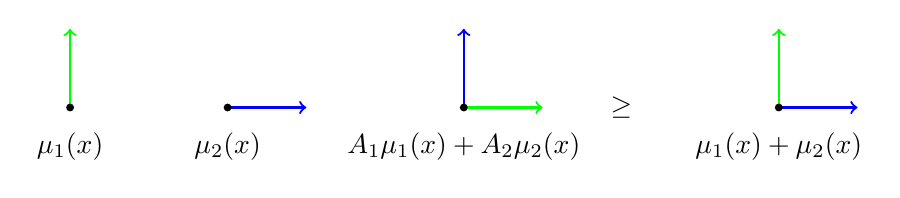
\begin{tikzpicture}
      \begin{scope}[shift={(-7,0)}]
        \draw[thick,->,green] (0,0) to (0,1);
        \fill (0,0) circle(.05);
        \node at (0,-.5) {$\mu_1(x)$};
      \end{scope}

      \begin{scope}[shift={(-5,0)}]
        \draw[thick,->,blue] (0,0) to (1,0);
        \fill (0,0) circle(.05);
        \node at (0,-.5) {$\mu_2(x)$};
      \end{scope}

      \begin{scope}[shift={(-2,0)}]
        \draw[thick,->,green] (0,0) to (1,0);
        \draw[thick,->,blue] (0,0) to (0,1);
        \fill (0,0) circle(.05);
        \node at (0,-.5) {$\pushf{A_{1}}{\mu_1(x)} + \pushf{A_{2}}{\mu_2(x)}$};
      \end{scope}

      \begin{scope}[shift={(0,0)}]
        \node at (0,0) {$\geq$};
      \end{scope}

      \begin{scope}[shift={(2,0)}]
        \draw[thick,->,green] (0,0) to (0,1);
        \draw[thick,->,blue] (0,0) to (1,0);
        \fill (0,0) circle(.05);
        \node at (0,-.5) {$\mu_1(x) + \mu_2(x)$};
      \end{scope}
    \end{tikzpicture}
    \caption{A representation of the optimal dual solution of \exemref{simple0} with the constraint \eqref{eq:dualinf1}.}
    \label{fig:simple0}
  \end{figure}

  A dual solution $\mu_1$ (resp. $\mu_2$)\footnote{In the arbitrary switching case, we write $\mu_\sigma$ instead of $\mu_{uv\sigma}$ for short}
  for the first (resp. second) matrix has the measure $\mu_1 = \delta_{(0,1)}/2$ (resp. $\mu_2 = \delta_{(1,0)}/2$).
  This is the solution obtained by applying \lemref{traj2meas} to the cycle $(1, 2)$.
  This is shown in \figref{simple0}.

\end{myexem}

\begin{myrem}
  Occupation measures for continuous switched systems are studied in \cite{claeys2016modal}.
  These measures are supported on the cartesian product of the state space and a finite interval of time $t \in [0, T]$
  while in this paper, the measures are only supported on the subset $\Sn$ of the state space.
  Indeed, since the system \eqref{eq:switchsys} is homogeneous and time-invariant, we can encode trajectories in a measure on $\Sn$ (\lemref{traj2meas}) and
  still be able to recover it (\cororef{instabcert}).

  The measures studied in \cite{hare2011explicit} are supported on the paths in $\G$.
  They are related to the measures studied in this paper since given a cycle $c$,
  we can compute the occupation measures of the trajectory using this switching cycle and starting with a leading eigenvector of $A_c$ as $x_0$ with \lemref{traj2meas}.
\end{myrem}



One may wonder whether \lemref{traj2meas} also works in the reverse direction to give a \emph{constructive} proof for \cororef{instabcert} when the measures $\mu_{uv\sigma}$ are atomic.
Namely, can we extract a periodic trajectory of period $c$ with $\jsrc \geq \gamlb$ from any atomic feasible solution of \progref{dualinf} with $\gamlb$.
As such solution may be the convex hull of solutions obtained by the construction of \lemref{traj2meas}, we may recover several periodic trajectory, from which there might be only one that satisfies $\jsrc \geq \gamlb$.
The following Lemma provides a constructive way to recover a periodic trajectory of period $c$ satisfying $\jsrc \geq \gamlb$ in the scalar case%
\footnote{Note that in this case, any measure is atomic since $\Sn$ is zero-dimensional}%
, i.e. $n = 1$%





\begin{lemma}
  \label{lem:instabcerts}
  Consider \defAGs{}.
  If there exists a feasible solution $\mu$ of \progref{dualinf} with $\gamlb$,
  then there exists a cycle $c$ with $\jsrc \geq \gamlb$.
  \begin{proof}
    Let $(\mu, \gamma)$ be the solution.
    By \eqref{eq:dualinf3} and \eqref{eq:dualinf1}, we can find a cycle $c$ for which each edge $e$ has a nonzero measure $\mu_e$.

    If $\jsrc \geq \gamma$, we are done.
    Otherwise, if $\jsrc < \gamma$, using \lemref{traj2meas},
    we can build a feasible solution $\nu$ such that \eqref{eq:dualinf1} is satisfied with equality for $\gamlb = \jsrc$.
    This means that $\mu - \lambda \nu$ is feasible with $\gamma$ for any $\lambda \geq 0$ such that $\mu - \lambda \nu \geq 0$.
    Let $\opt{\lambda}$ be the maximum value of $\lambda$ such that $\mu - \lambda \nu \geq 0$.
    Since $n = 1$, $\Sn$ is zero dimensional so for at least one edge $e$ of the cycle $c$, $\mu_e - \opt{\lambda} \nu_e$ is zero.
    Moreover, since $\mu_e$ is nonzero for all edge $e$ of the cycle, $\lambda > 0$.
    Therefore, the number of edges with nonzero measure has decreased and at least one of the constraints \eqref{eq:dualinf1} is now satisfied with strict inequality.

    This process can only be repeated finitely many times until $\mu$ becomes the trivial solution since the number of edges with nonzero measure decrease each time.
    Moreover we will have $\jsrc \geq \gamma$ at least once since the constraints \eqref{eq:dualinf1} cannot be satisfied with strict inequality for the trivial solution.
  \end{proof}
\end{lemma}

Given a feasible solution of \progref{dualinf} and a common partition of the support of the measures,
we show in \propref{Bsc} how to transform the solution into a solution of a scalar switched system.
Using this transformation, we can always recover a cycle $c$ for which $\jsrc = \gamma$ from a solution of \progref{dualinf} with $\gamlb = \gamma$ for which the measures are atomic.

\begin{proposition}
  \label{prop:Bsc}
  Consider \defAGe.
  Suppose that there exists a feasible solution $\mu$ of \progref{dualinf} with $\gamlb = \gamma$
  and a finite family $\mathcal{S}$ of disjoint subsets of $\Sn$ such that
  the support of each measure is included in the union of the sets of the family $\mathcal{S}$.
  Then there exists sets $B_1, \ldots, B_k \in \mathcal{S}$ and a cycle $\sigma_1, \ldots, \sigma_k$ of $\G$ such that
  \[ \prod_{i=1}^k \max_{x \in B_i} \|A_{\sigma_i} x\|_2 \geq \gamma^k \]
  and $A_{\sigma_i} B_i \cap B_{i+1} \neq \emptyset$ for $i=1, \ldots, k$ where $B_{k+1}=B_1$.
  \begin{proof}
    Given a set $B \in \mathcal{S}$ and an \arc{} $e \in \Arcs$, let $\mu_e^B$ denote the measure defined as $\mu_e^B(C) = \mu_e(C \cap B)$.
    We consider a new constrained switched system with matrices $\A' \subseteq \R^{1 \times 1}$ and automaton $\G'(\Nodes', \Arcs')$
    where $\Nodes' = \{\, (v,B) \mid v \in \Nodes, B \in \mathcal{S} \,\}$,
    $e'((u,v,\sigma), B, C) = ((u,B), (v,C), (\sigma,B))$,
    $\Arcs' = \{ e'(e, B, C) \mid e \in \Arcs, B, C \in \mathcal{S}, A_e B \cap C \neq \emptyset \}$,
    and $A'_{(\sigma,B)} = \max_{x \in B} \|A_\sigma x\|_2$.
    From any solution $\mu$ of the original system feasible for $\gamlb$, the following solution of the system with matrices $\A'$ and automaton $\G'$
    \[ \mu'_{e'(e,B,C)} = \frac{(\pushf{A_e}{\mu_e^B})(C)}{(\pushf{A_e}{\mu_e^B})(\Sn)} \mu_e(B) \]
    is also feasible with $\gamlb$.
    Indeed, by construction, for any $v \in \Nodes, C \in \mathcal{S}$, we have
    \begin{align}
        \label{eq:lhstransfer}
        \begin{split}
        \sum_{e \in \Arcsin_{1}(v), B \in \mathcal{S}} (\pushf{A_e}{\mu_e^B})(C)
        & =
        \sum_{e \in \Arcsin_{1}(v), B \in \mathcal{S}} \mu_{e'(e, B, C)}' \frac{(\pushf{A_e}{\mu_e^B})(\Sn)}{\mu_e(B)}\\
        & \stackrel{\eqref{eq:pushfineq}}{\leq}
        \sum_{e \in \Arcsin[\Arcs']_1(v, C)} \pushf{A'_{e}}{\mu_{e}'}
        \end{split}\\
        \label{eq:rhstransfer}
        \begin{split}
        \sum_{e \in \Arcsout_1(v)} \mu_e(C)
        & =
        \sum_{e \in \Arcsout_1(v), D \in \mathcal{S}} \frac{(\pushf{A_e}{\mu_e^C})(D)}{(\pushf{A_e}{\mu_e^C})(\Sn)} \mu_e(C)\\
        & =
        \sum_{e \in \Arcsout[\Arcs']_1(v, C)} \mu_{e}'.
        \end{split}
    \end{align}
    By \eqref{eq:dualinf1} on $\mu$, the left-hand side of \eqref{eq:rhstransfer} is smaller than
    the left-hand side of \eqref{eq:lhstransfer}.
    Therefore, the right-hand side of \eqref{eq:rhstransfer} is smaller than the right-hand side of \eqref{eq:lhstransfer}
    hence $\mu'$ satisfies \eqref{eq:dualinf1} on the new switched system.

    Therefore, by \lemref{instabcerts},
    there is a cycle $(\sigma_1, B_1), \ldots, (\sigma_k, B_k)$ of $\G'$ such that the modes $\sigma_i$ and sets $B_i$ are as required.
  \end{proof}
\end{proposition}

\begin{myexem}
  \label{exem:simple05}
  Consider the dual solution obtained in \exemref{simple0}.

  The supports of $\mu_1$ and $\mu_2$ are respectively $B_1 = \{(0, 1)\}$ and $B_2 = \{(1, 0)\}$.
  The automaton $G'(V', E')$ obtained by the transformation of \propref{Bsc} is defined by
  $V' = \{(1, B_1), (1, B_2)\}$ and $E' = \{((1, B_1), (1, B_2), (1, B_1)), ((1, B_2), (1, B_1), (2, B_2))\}$.
  The new $1 \times 1$ matrices are $A'_{(1, B_1)} = 1$ and $A'_{(2, B_2)} = 1$.

  The computation of the CJSR of this scalar system is a \emph{maximum cycle mean} problem
  as outlined in \cite{ahmadi2012joint}.
  The cycle of maximum geometric mean is $((1, B_1), (2, B_2))$ which geometric mean $\sqrt{1 \cdot 1} = 1$.
  We recover the cycle $(1, 2)$ found in \exemref{simple0}.
\end{myexem}
